\documentclass{article}
\usepackage{tikz,pgfplots}
%\pgfplotsset{colormap={name}{
%	color(0cm)=(blue);
%	color(1cm)=(green);
%	color(2cm)=(yellow)
%	color(3cm)=(red)}}
\pgfplotsset{colormap={blues}{
       color(0cm)=(white);
       color(1cm)=(blue)}}

\definecolor{diplom1}{rgb}{0.0 0.4 1.0}
\definecolor{diplom2}{rgb}{0.0 0.0 0.6}
\definecolor{diplom3}{RGB}{153,0,0} %unirot
\definecolor{diplom4}{RGB}{232,215,23}
\definecolor{diplom5}{RGB}{51,37,60}

\definecolor{unirot}{RGB}{153,0,0}
\definecolor{unirot_hell}{RGB}{255,228,225}
\definecolor{lightblue}{RGB}{242.2,249.88,255}

\begin{document}
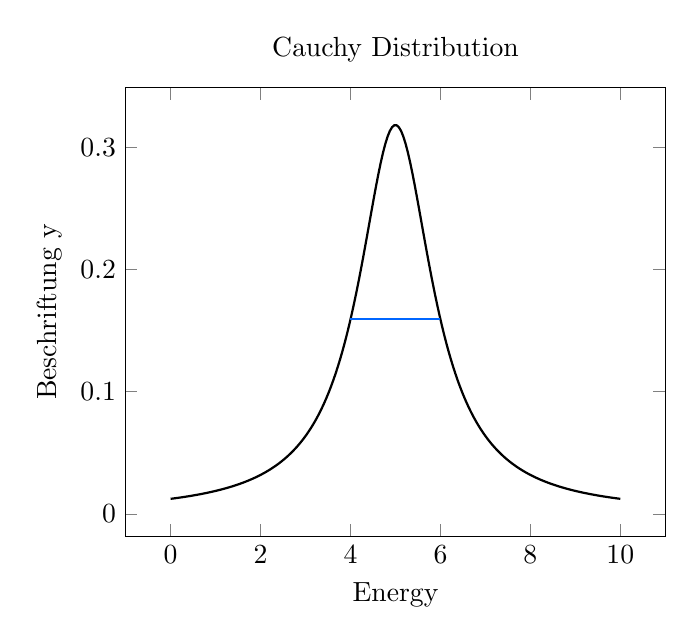
\begin{tikzpicture}

\begin{axis}[
             domain=0.00:10.00,
             xlabel={Energy},
             ylabel={Beschriftung y},
             title={Cauchy Distribution},
             samples=200
             ]

	
\addplot[
         thick
	]
        {1.0/3.14159 * 1.0/((x-5)^2+1.0^2)};
  \draw[-,thick,diplom1] (axis cs:4.0,0.15915) -- (axis cs:6,0.15915);
		
\end{axis}
\end{tikzpicture}

 \begin{tikzpicture}[
          scale=1.0,>=stealth,domain=0.5:10,samples=100,
          declare function={
          gamma = 1.0;
          factor = 16.0;
          halfmax = factor * 0.15915;
          x_0 = 5.0;
          distrib(\x) = factor/3.14159 * gamma / ((\x-x_0)^2 + gamma^2);
        }]
%     \tiny
%  \draw[very thin,color=gray] (-0.1,-0.1) grid (4.9,4.9);
  \draw[->,thick] (-0.2,0) -- (10.2,0) node[right] {$x$};
  \draw[->,thick] (0,-0.2) -- (0,7.2) node[above] {$f(x,x_0,\gamma)$};
  % add ticks
  \draw [thick] (5,0) -- (5,-5pt) node [anchor=north] {$x_0$};

  \draw [color=black,domain=0:10,smooth,very thick]    plot
         (\x,{distrib(\x)});% node [anchor=south] {Cauchy distribution};
  \draw [-,very thick,diplom1] (4.0,halfmax) -- (6,halfmax)
         node [anchor=south west] {$2\gamma$};
 \end{tikzpicture}


	\end{document}
